% imports 
\section{Overview}
Previous solutions to the bus charge problem have all struggled with scalability where scalable is defined as a solution where the runtime and cost increase linearly with the number of buses. In this work, we propose a solution which scales to a large number of buses by segmenting the problem into a series of sub-problems belonging to one of three groups as shown in Fig. \ref{fig:processChain}. 
\par Each sub-problem is solved using a linear, quadratic, or integer program and when used together the series of programs provides a near optimal charge plan. Each sub-problem addresses elements from one of three areas: energy allocation and bus grouping, session length and bus-to-charger assignments, and second-by-second optimization.
\subsection{Energy Allocation and Group Assignment}
\par The first set of problems answers two primary questions: At which time should energy be delivered to each bus and which buses' are most able to share chargers and contains three sub-problems: Unconstrained charge schedule, Smooth charge schedule, and group separation. 
\par The unconstrained schedule problem from Section \ref{sec:unconstrainedSchedule} computes an optimal charge schedule which minimises the monthly cost of power in the presence of uncontrolled loads under the assumption that each bus maintains a dedicated charger. 
\par The smooth schedule problem from Section \ref{sec:unconstrainedSmoothSchedule} has the same form as the unconstrained scheduling problem with two differences: The monthly cost is required to match the optimal cost from the solution to the unconstrained scheduling problem and the objective for the smooth schedule problem penalizes change in the scheduled charge rates.
\par The group assignment problem from Section \ref{sec:groupAssignment} uses the resulting charge schedules from the solution to the smooth schedule problem to separate buses into groups where each bus's schedule overlaps as little as possible with the other schedules for buses in the same group so that each group can be addressed separately to manage the number of computations in succeeding problems.
\subsection{Session Time and Charger Assignment}
The problems in the session time and charger assignment section are computed on a per-group basis to reduce the number of computations, address the questions of when should charge sessions start and stop, and on which charger should each session occur and are comprised of three sub-problems: De-Fragmentation, charger assignment, and session refinement.
\par The defragmentation problem from Section \ref{sec:defragmentation} attempts to consolidate charge sessions with small amounts of energy to reduce the number of charge sessions and serves to both decrease the computational complexity of the charger assignment problem by reducing the number of charge sessions and simplify the charge schedule to make it more operationally feasible.
\par After consolidation, each charge session is defined by a minimum/maximum start/stop time as given by the bus's arrival and departure times and an energy requirement in kW. The charger assignment problem from Section \ref{sec:chargerAssignment} uses the availability and energy constraints to assign chargers to charge sessions.
\par Once charge sessions are placed, the final step is to ensure each session makes the most of each charger's availability. Many times, especially when using non-optimal gaps in the charger assignment problem, the charge schedules may not use all available time on a charger. The charger refinement problem expands each charge session to fill unused time on either side and prioritizes sessions with higher energy demands for adjacent sessions.
\subsection{Final Optimization}
Solutions to the previous problems provide us with a set of charge sessions, energy requirements, and time schedules for specific chargers. The final question to be answered is how should the energy for each session will be delivered. The two sub-problems in the final optimization section mirror the first two problems from the Energy Allocation and Group Assignment section. The first uses the energy and time constraints from previos solutions to compute an optimal charge schedule in Section \ref{sec:constrainedSchedule} and is analagous to the unconstrained charge problem. The second computes a smoothed charge schedule with the same cost as the constrained schedule solution in Section \ref{sec:constrainedSmoothSchedule} and is analagous to the Smooth charge schedule problem in Section \ref{sec:unconstrainedSmoothSchedule}.
\begin{figure*}\centering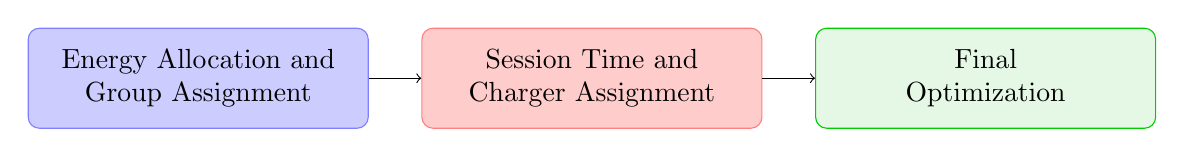
\begin{tikzpicture}
	\node[rectangle, draw=blue!50, fill=blue!20, minimum width=1.7in, minimum height=0.5in, rounded corners](set1) at (0,0) {\begin{tabular}{c} Energy Allocation and\\ Group Assignment\end{tabular}}; 
	\node[rectangle, draw=red!50, fill=red!20, minimum width=1.7in, minimum height=0.5in, rounded corners](set2) at (5,0) {\begin{tabular}{c} Session Time and \\Charger Assignment \end{tabular}}; 
	\node[rectangle, draw=green!80!black, fill=green!70!black!10, minimum width=1.7in, minimum height=0.5in, rounded corners](set3) at (10,0) {\begin{tabular}{c} Final \\ Optimization\end{tabular}}; 
	\draw[->] (set1.east) -- (set2.west);
	\draw[->] (set2.east) -- (set3.west);
\end{tikzpicture}\caption{Overall Processing Chain}\label{fig:processChain}\end{figure*}


\begin{figure*}\centering\scalebox{0.8}{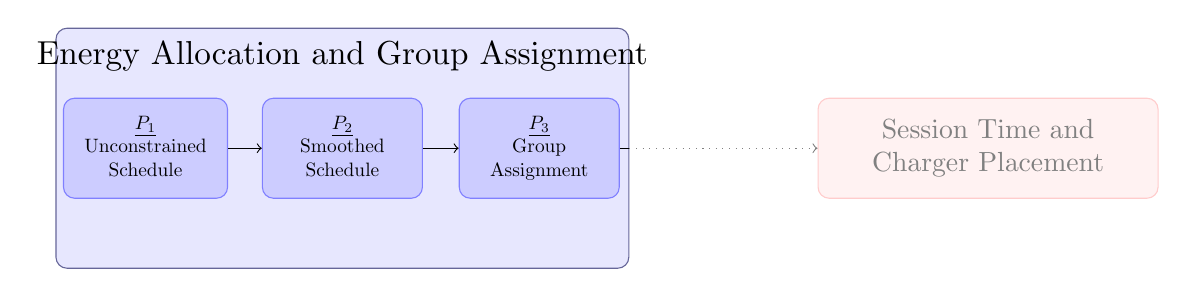
\begin{tikzpicture}
\node[rectangle, draw=gray!80!blue, fill=gray!10!blue!10, minimum width=\textwidth*0.6, minimum height=1.2in, rounded corners, label={[label distance=-0.67cm]above:\scalebox{1.2}{Energy Allocation and Group Assignment}}](outline) at (0,0){};
	\node[rectangle, draw=blue!50, fill=blue!20, minimum width=0.8in, minimum height=0.5in, rounded corners](problem1) at (-2.5,0) {\scalebox{0.7}{\begin{tabular}{c} \underline{$P_1$} \\ Unconstrained \\ Schedule\end{tabular}}}; 
	\node[rectangle, draw=blue!50, fill=blue!20, minimum width=0.8in, minimum height=0.5in, rounded corners](problem2) at (0,0) {\scalebox{0.7}{\begin{tabular}{c}\underline{$P_2$} \\  Smoothed \\ Schedule\end{tabular}}}; 
	\node[rectangle, draw=blue!50, fill=blue!20, minimum width=0.8in, minimum height=0.5in, rounded corners](problem3) at (2.5,0) {\scalebox{0.7}{\begin{tabular}{c}\underline{$P_3$} \\ Group \\ Assignment\end{tabular}}}; 
	\node[rectangle, draw=red!20, fill=red!5, text=black!50, minimum width=1.7in, minimum height=0.5in, rounded corners](problem4) at (8.2,0){\begin{tabular}{c}Session Time and \\ Charger Placement\end{tabular}};
	\draw (problem3.east) -- (outline.east);
	\draw[->, draw=black!50, dotted] (outline.east) -- (problem4.west);
	\draw[->, draw=black] (problem1.east) -- (problem2.west);
	\draw[->, draw=black] (problem2.east) -- (problem3.west);
\end{tikzpicture}}\caption{Processing chain for the energy allocation and group assignment problems} \label{fig:set1Chain}\end{figure*}


\begin{figure*}\centering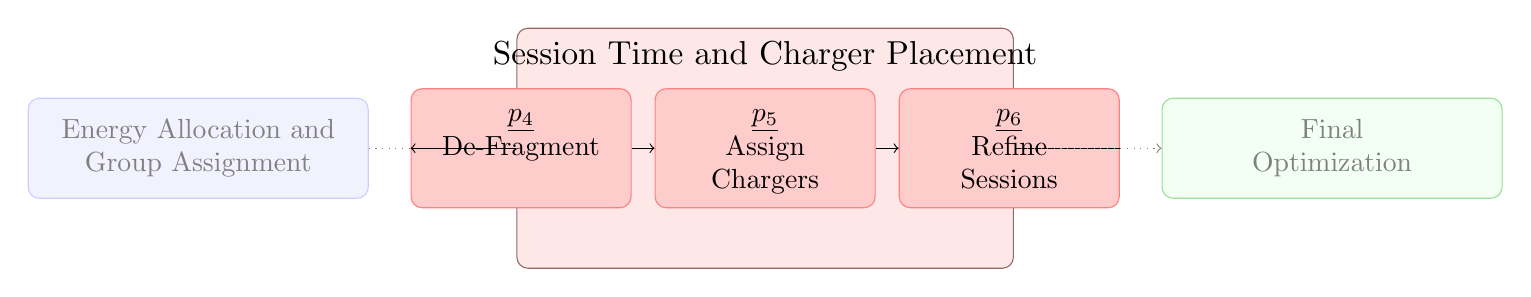
\begin{tikzpicture}
\node[rectangle, draw=gray!80!red, fill=gray!10!red!10, minimum width=\textwidth*0.52, minimum height=1.2in, rounded corners, label={[label distance=-0.67cm]above:\scalebox{1.2}{Session Time and Charger Placement}}](outline) at (0,0){};
	\node[rectangle, draw=red!50, fill=red!20, minimum width=1.1in, minimum height=0.5in, rounded corners](problem1) at (-3.1,0) {\begin{tabular}{c} \underline{$p_4$} \\ De-Fragment \\  \\\end{tabular}}; 
	\node[rectangle, draw=red!50, fill=red!20, minimum width=1.1in, minimum height=0.5in, rounded corners](problem2) at (0,0) {\begin{tabular}{c}\underline{$p_5$} \\ Assign\\ Chargers\end{tabular}}; 
	\node[rectangle, draw=red!50, fill=red!20, minimum width=1.1in, minimum height=0.5in, rounded corners](problem3) at (3.1,0) {\begin{tabular}{c}\underline{$p_6$} \\ Refine\\ Sessions\end{tabular}}; 
	\node[rectangle, draw=blue!20, fill=blue!5, text=black!50, minimum width=1.7in, minimum height=0.5in, rounded corners](problem0) at (-7.2,0){\begin{tabular}{c}Energy Allocation and\\ Group Assignment\end{tabular}};
	\node[rectangle, draw=green!70!black!40, fill=green!5, text=black!50, minimum width=1.7in, minimum height=0.5in, rounded corners](problem4) at (7.2,0){\begin{tabular}{c}Final \\ Optimization\end{tabular}};
	\draw[draw=black!50, dotted] (problem0.east) -- (outline.west);
	\draw[->] (outline.west) -- (problem1.west);
	\draw (problem3.east) -- (outline.east);
	\draw[->, draw=black!50, dotted] (outline.east) -- (problem4.west);
	\draw[->, draw=black] (problem1.east) -- (problem2.west);
	\draw[->, draw=black] (problem2.east) -- (problem3.west);
\end{tikzpicture}\caption{Processing chain for each group} \label{fig:set2Chain}\end{figure*}


\begin{figure*}\centering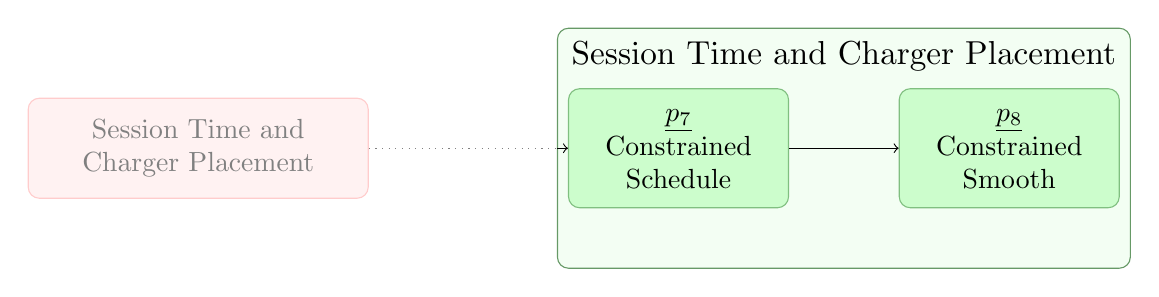
\begin{tikzpicture}
\node[rectangle, draw=gray!80!green, fill=gray!10!green!5, minimum width=\textwidth*0.6, minimum height=1.2in, rounded corners, label={[label distance=-0.67cm]above:\scalebox{1.2}{Session Time and Charger Placement}}](outline) at (0,0){};
	\node[rectangle, draw=green!50!black!50, fill=black!3!green!20, minimum width=1.1in, minimum height=0.5in, rounded corners](problem1) at (-2.1,0) {\begin{tabular}{c} \underline{$p_7$} \\ Constrained \\ Schedule\end{tabular}}; 
	\node[rectangle, draw=green!50!black!50, fill=black!3!green!20, minimum width=1.1in, minimum height=0.5in, rounded corners](problem3) at (2.1,0) {\begin{tabular}{c}\underline{$p_8$} \\ Constrained \\ Smooth\end{tabular}}; 
	\node[rectangle, draw=red!20, fill=red!5, text=black!50, minimum width=1.7in, minimum height=0.5in, rounded corners](problem0) at (-8.2,0){\begin{tabular}{c}Session Time and \\ Charger Placement\end{tabular}};
	\draw[draw=black!50, dotted] (problem0.east) -- (outline.west);
	\draw[->] (outline.west) -- (problem1.west);
	\draw[->, draw=black] (problem1.east) -- (problem3.west);
\end{tikzpicture}\caption{Processing chain for the Final Optimization set} \label{fig:set3Chain}\end{figure*}


\section{Unconstrained Schedule \label{sec:unconstrainedSchedule}}
This section describes a program that finds an optimal charge schedule where buses are allowed to charge without regard to the number of available chargers. This solution is considered ``optimal'' and will be used in later sections to formulate a feasible solution that accounts for the number of chargers.
\begin{table*}
\centering
\caption{Description of the billing structure}
\begin{tabular}{c | c c c}
		                   & On-Peak                & Off-Peak               & Facilities (Both)\\ \hline
		Energy Rate        & \$ 0.058282  /kWh & \$ 0.029624 /kWh  & None \\
		Energy Rate Symbol & $\mu_{\text{e-on}}$    & $\mu_{\text{e-off}}$   & None \\ \hline
		Power Rate  & \$ 15.73 /kW           & None                   & \$ 4.81 /kW \\
		Power Rate Symbol  & $\mu_{\text{p-on}}$    & None            & $\mu_{\text{p-all}}$
	\end{tabular}
	\label{tab:charges} 
\end{table*}

 
\begin{figure*}
\centering
\scalebox{0.8}{
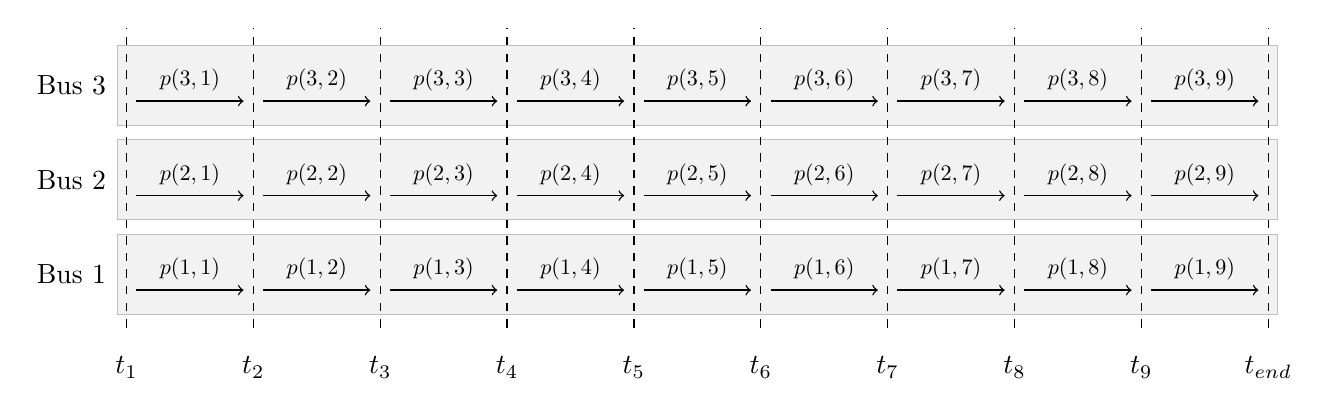
\begin{tikzpicture}
	\node[rectangle, draw=gray!50, fill=gray!10, minimum width=5.8in, minimum height=0.4in](bus1Box) at (7.75,0.8){};
	\node(bus1BoxLabel) at (-0.2, 0.8){Bus 1}; 
	
	\node[rectangle, draw=gray!50, fill=gray!10, minimum width=5.8in, minimum height=0.4in](bus2Box) at (7.75,2){};
	\node(bus1BoxLabel) at (-0.2, 2.0){Bus 2};
	
	\node[rectangle, draw=gray!50, fill=gray!10, minimum width=5.8in, minimum height=0.4in](bus3Box) at (7.75,3.2){};
	\node(bus1BoxLabel) at (-0.2, 3.2){Bus 3};
	
	\foreach \curLab/\preLab[count=\c, evaluate=\c as \pos using {0.5 + (\c - 1)*14.5/9}] in {t_1/t_1, t_2/t_1, t_3/t_2, t_4/t_3, t_5/t_4, t_6/t_7, t_7/t_6, t_8/t_7, t_9/t_8, t_{end}/t_9}
	{
		\node[label=below:$\curLab$](b\c) at (\pos, 0){};
		\node(t) at (\pos, 3.8){};
		\draw[dashed, line width=0.5pt] (b\c.north) -- (t.north); 
		\ifnum\c>1 
			\node(b1Curr) at (\pos, 0.8 - 0.2){};
			\node(b2Curr) at (\pos, 2.0 - 0.2){};
			\node(b3Curr) at (\pos, 3.2 - 0.2){};
			\def\temp{\number\numexpr\c - 1}
			\draw[->, line width=0.5pt] (b1Prev.east) -- node[midway, above]{\scalebox{0.8}{$p(1,\temp)$}}(b1Curr.west);
			\draw[->, line width=0.5pt] (b2Prev.east) -- node[midway, above]{\scalebox{0.8}{$p(2,\temp)$}}(b2Curr.west);
			\draw[->, line width=0.5pt] (b3Prev.east) -- node[midway, above]{\scalebox{0.8}{$p(3,\temp)$}}(b3Curr.west);	
		\fi
			\node(b1Prev) at (\pos, 0.8 - 0.2){};
			\node(b2Prev) at (\pos, 2.0 - 0.2){};
			\node(b3Prev) at (\pos, 3.2 - 0.2){};	
	}
	\path (b9.south) -- node[midway, below=0.1in]{$\hdots$}(b10.south);

\end{tikzpicture}}
\caption{Demonstrates how bus power use is conceptualized}
\label{fig:busPower}
\end{figure*}


\begin{figure*}
\centering
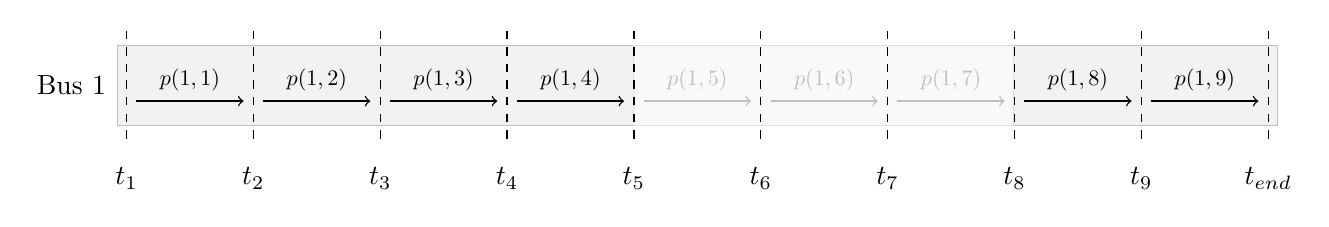
\begin{tikzpicture}
	\node[rectangle, draw=gray!50, fill=gray!10, minimum width=5.8in, minimum height=0.4in](bus1Box) at (7.75,0.8){};
	\node(bus1BoxLabel) at (-0.2, 0.8){Bus 1}; 
	\node[rectangle, draw=gray!25, fill=gray!5, minimum width=1.9in, minimum height=0.4in](bus1Box) at (7.75 + 1.6,0.8){};
	
	\foreach \curLab/\preLab[count=\c, evaluate=\c as \pos using {0.5 + (\c - 1)*14.5/9}] in {t_1/t_1, t_2/t_1, t_3/t_2, t_4/t_3, t_5/t_4, t_6/t_5, t_7/t_6, t_8/t_7, t_9/t_8, t_{end}/t_9}
	{
		\node[label=below:$\curLab$](b\c) at (\pos, 0){};
		\node(t) at (\pos, 1.4){};
		\ifnum\c>1 
			\node(b1Curr) at (\pos, 0.8 - 0.2){};
				\ifnum\c > 5
					\ifnum\c < 9 
						\def\clr{black!25}
					\else
						\def\clr{black}
					\fi
				\else
					\def\clr{black}
				\fi
				\draw[->, line width=0.5pt, \clr] (b1Prev.east) -- node[midway, above]{\scalebox{0.8}{$p(1,\number\numexpr\c-1)$}}(b1Curr.west); 
		\fi
		\node(b1Prev) at (\pos, 0.8 - 0.2){};
		\draw[dashed, line width=0.5pt] (b\c.north) -- (t.north); 
	}
	\path (b9.south) -- node[midway, below=0.1in]{$\hdots$}(b10.south);

\end{tikzpicture}
\caption{Bus schedule with availability}
\label{fig:busAvail}
\end{figure*}

 
\subsection{Formulation \label{sec:formulation}} 
The cost objective that we desire to minimize is modeled after \cite{rocky_mountain_power_rocky_2021}, which contains two primary elements: the cost of energy, and power demand. Energy is billed per kWh for on-peak and off-peak hours. The on-peak rate is more expensive because there is generally more demand for power during this time, whereas off-peak hours tend to be less expensive. The demand is covered in two separate chargers.  The first is a facilities charge which is billed per kW for the highest 15-minute average power use over the course of the month. The second is a demand charge, which is also billed per kW, but is only billed for the highest 15-minute average power usesd during on-peak hours. The rates for each component are given in Table \ref{tab:charges}.  

Before we may compute the total monthly cost of electricity, we must define expressions for the average power and energy over time.  Let each day be divided into 15-minute intervals for each bus where the average power expended for bus $i$ during time $j$ is denoted $p(i,j)$ as shown in Fig. \ref{fig:busPower}. The resulting solution of the program we will develop will yield the average power expended by each bus during each period of time.
\par One constraint for which the solution must account is bus availability.  When a bus is out of the station, the maximum average power for that time must be zero. For example, if bus 1 were out on route for $t_5, t_6,$ and $t_7$, then the average power for those periods would be equal to zero as shown in Fig. \ref{fig:busAvail}. Let $\bm{b}_{p(i,j)}$ be the average power used by bus $i$ at time index $j$, and $\bm{b}$ be a vector which contains $b_{p(i,j)}$ for each bus and time index. Also let $\mathcal{A} \subset {i\times j}$  be the set of all indices where bus $i$ is in the station during time $t_j$ and $\tilde{\mathcal{A}}$ be its complement. Furthermore, let $p_{\text{max}}$ be the maximum power that a charger can deliver. 
\par We define a set of constraints so that buses do not use power when not in the station by letting
\begin{equation}\label{eqn:obj:power1}\begin{aligned}
	b_{p(i,j)} &= 0 \ \forall i,j \in \tilde{\mathcal{A}}  \\
	b_{p(i,j)} &\le p_{\text{max}} \ \forall i,j \in \mathcal{A} \\
	-b_{p(i,j)} &\le 0              \ \forall i,j \in \mathcal{A} 
\end{aligned}\end{equation}
\par The constraints in Eq. \ref{eqn:obj:power1} however to not account for buses that must charge for partial periods.  For example, if the day were divided into 15-minute time blocks, but a bus began charging at 10:07, then an average power of $p_{\text{max}}$ for that time slot would be inaccurate. Therefore, Eq. \ref{eqn:obj:power1} must be modified so that the average power for each block correctly reflects partial availability.  Let $\alpha(i,j)$ give the percentage of time that bus $i$ is available during time $j$. Eq. \ref{eqn:obj:power1} can be rewritten as
\begin{equation}\label{eqn:obj:power2}\begin{aligned}
	-b_{p(i,j)} &\le 0 \ \forall i,j \\
	b_{p(i,j)}  &\le p_{\text{max}}\cdot \alpha(i,j) \ \forall  i,j\\
\end{aligned}\end{equation}



